%
%  Labels
%
%  Created by Mustafa Youldash on 2014-04-25.
%  Copyright (c) 2014 Mustafa YOULDASH. All rights reserved.
%
\documentclass[12pt,a4paper,oneside,onecolumn]{article}

% .......................................... Preamble

% Include images and figures
\usepackage{graphicx}

% Use \usepackage[fleqn]{amsmath} to make the math environments left-aligned instead of centered
\usepackage[fleqn]{amsmath}

% .......................................... End

\begin{document}

	\section{Pictures}
	\label{sec:Pictures}

	\section{Referencing}

	I greeted in section \ref{sec:greetings}.

	\begin{figure}[htp]
		\centering
		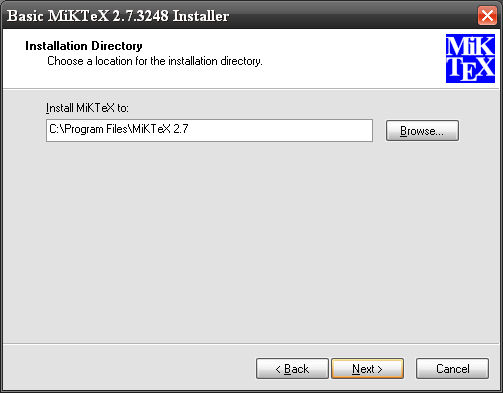
\includegraphics[scale=0.6]{Directory}
		\caption{Install Directory}
		\label{fig:directory}
	\end{figure}
	Figure \ref{fig:directory} shows a snapshot of an install phase.


	\section{Greetings}
	\label{sec:greetings}

	Hello!

	\clearpage

	\section{Formulas}
	\label{sec:Formulas}

	\begin{equation} \label{eq:solve}
	x^2 - 5 x + 6 = 0
	\end{equation}

	\begin{equation}
	x_1 = \frac{5 + \sqrt{25 - 4 \times 6}}{2} = 3
	\end{equation}

	\begin{equation}
	x_2 = \frac{5 - \sqrt{25 - 4 \times 6}}{2} = 2
	\end{equation}

	and so we have solved equation \ref{eq:solve}

\end{document}
